\documentclass[fleqn,10pt]{wlscirep}
\usepackage[utf8]{inputenc}
\usepackage[T1]{fontenc}
\title{NMRlipids Databank}

\author[1,*]{Anne Kiirikki}
\author[1,*]{O. H. Samuli Ollila}
%\author[1,2,+]{Christine Author}
%\author[2,+]{Derek Author}
\affil[1]{University of Helsinki, Institute of Biotechonology, Helsinki, Finland}
%\affil[2]{Affiliation, department, city, postcode, country}

\affil[*]{samuli.ollila@helsinki.fi}

%\affil[+]{these authors contributed equally to this work}

%\keywords{Keyword1, Keyword2, Keyword3}

\begin{abstract}
We present a databank of lipid bilayer simulations from the NMRlipids open collaboration project.
\end{abstract}
\begin{document}

\flushbottom
\maketitle
% * <john.hammersley@gmail.com> 2015-02-09T12:07:31.197Z:
%
%  Click the title above to edit the author information and abstract
%
\thispagestyle{empty}

%\noindent Please note: Abbreviations should be introduced at the first mention in the main text – no abbreviations lists. Suggested structure of main text (not enforced) is provided below.

\section{Introduction}

The demand for sharing and reusing of MD simulation data is increasing, but practical solution remains unclear due to unsolved issues in data storage and indexing.
Here we present a solution for lipid bilayers based on overlay databank structure.

%The Introduction section, of referenced text\cite{Figueredo:2009dg} expands on the background of the work (some overlap with the Abstract is acceptable). The introduction should not include subheadings.

\section{Results}

%Up to three levels of \textbf{subheading} are permitted. Subheadings should not be numbered.

\subsection{Quality evaluation of force fields}

The quality of each simulation is evaluated against NMR order parameters.
Indexing of experimental data to automatize evaluation is currently in progress by Anne Kiirikki.

\subsection{Water permeability across membranes}

Averaging water density profiles over all simulations in the databank enables us to calculate the barrier for the water penetration through lipid bilayers.

\subsection{Spin relaxation rates of confined water close to membranes}

Usefulness of the databank beyond MD simulation experts is demonstrated by analysing water spin relaxation times close to bilayers which are used in MRI imaging.

%Example text under a subsection. Bulleted lists may be used where appropriate, e.g.

%\begin{itemize}
%\item First item
%\item Second item
%\end{itemize}

%\subsubsection*{Third-level section}
 
%Topical subheadings are allowed.

\section{Discussion}

%The Discussion should be succinct and must not contain subheadings.

\section{Methods}

%Topical subheadings are allowed. Authors must ensure that their Methods section includes adequate experimental and characterization data necessary for others in the field to reproduce their work.

\subsection{Structure of the databank}

NMRlipids databank is a overlay databank composed of index files containing information on the location of original data and all essential information on simulations needed in further use and automatic analysis. Each simulation system is identified using the hash of original trajectory and topology file. The index files are stored in folder structure based on the identity codes of the simulations.

\subsection{Analysis of the data in databank}

Index files in the datanbank contain all the essential information to perform analyses from the simulations. Systems under interest can be selected automatically browsing the index files and filtering the desired properties. 

Analysis results can be most conveniently stored to a new datanbank with identical indexing as the original databank. The results can be then easily shared and browsed indentically to the original databank.

\subsection{Indexing the simulation data}

%\subsubsection*{AddData.py}
AddData.py is a script that builds a database that contains a dictionary file and analysis data of each simulation. The dictionary file contains information about the simulation. The script also calculates order parameters of all CH bonds of the lipids in the simulation. To add a simulation it must be first uploaded to Zenodo (www.zenodo.org). The trajectory and topology files of the simulation are downloaded to the working directory from Zenodo but these are not saved into the database. To add a simulation to the database the user has to give some essential information about the simulation. This is done by writing a info file (*INFO.yaml) which is passed to AddData.py. 
\newline \\
AddData.py requires GROMACS and MDAnalysis library to be installed.
\newline \\
Run AddData.py as follows:
\newline \\
python3 AddData.py -f exampleINFO.yaml
\newline \\
There is also a script runAddData.sh that can be used to loop over several info files to add many simulations at one go.

%\subsubsection*{Simulation dictionary}
A simulation dictionary contains information about the simulation. Some of the information is provided by the user. The numbers of lipid molecules, solvent and ions are automatically read from the files and so are the simulation temperature and trajectory length. All this information is saved to a file named README.yaml.



\subsubsection{Compulsory user input}
The following parameters are compulsory and have a strict format.

\subsubsection*{DIR\_WRK}
DIR\_WRK is the path of the working directory.

\subsubsection*{DOI}
DOI is the DOI access number of the simulation. Use the version DOI on Zenodo.

\subsubsection*{MAPPING\_DICT}
MAPPING\_DICT is a dictionary that contains the mapping file names for each lipid in the membrane. For each entry in the dictionary the key is the lipid name and the value is the name of the mapping file. The existing mapping files are in the directory named "mapping\_files". If a mapping file of a certain lipid does not exist the user must construct it.
\newline \\
The purpose of a mapping file is to circumvent the problem caused by different atom naming conventions used by different force fields. The first column of a mapping file contains general atom names. The second column contains the name of the atom as it is in the force field. If the lipid consists of several residues which is the case in some AMBER force fields, then a third column is needed which contains the name of the residue to which each atom belongs to.

\subsubsection*{SOFTWARE}
SOFTWARE stands for the name of the software used for running the simulation. The options are GROMACS, AMBER, NAMD, CHARMM and OPENMM. So far, only simulations run with GROMACS are accepted by the script.

\subsubsection*{TRJ}
TRJ stands for the name of the trajectory file.
\subsubsection*{TPR}
TPR stands for the name of the topology file.

\subsubsection*{PREEQTIME}
PREEQTIME means the time used for pre-equilibrating the system. This should be in nano seconds. 
\subsubsection*{TIMELEFTOUT}
TIMELEFTOUT stands for the length of the simulation in nano seconds to be left out at the beginning of the simulation. This value is used in the script to discard the given length from the analysis!

\subsubsection*{UNITEDATOM}
The handling of united atom simulations is enabled by a separate script called buildH\_calcOP.py. In case of a united atom simulation, the user has to give the names of the lipids and the corresponding names of those lipids as they are in the dic\_lipids.py dictionary used by buildH\_calcOP.py script. In the case of an all atom simulation this can be given as an empty string.

\subsubsection*{Molecule names}
The databank has default names for lipids, ions and solvent. The user must also provide the names of the molecules, ions and solvent that are used in the simulation to match the names used by the databank. The names provided by the user must be the same as in the tpr file. If a lipid consists of more than one residue the name of the head group residue is given. If the name of the molecule is not in the databank it needs to be added. The names of the molecules are listed in dictionaries called lipids\_dict and molecules\_dict which are in the script. If a new molecule is added it needs to be added to molecule\_numbers\_dict and molecule\_ff\_dict too.

%%%%%%%%%%%%%%%%%%%%%%%%%%%%%%free form parameters%%%%%%%%%%%%%%%%%%%%%%%%%%%%%%%%%%%%%%%%%
\subsubsection{Optional and free form user input}
The form of how the values of these parameters are written is not essential for the script to work properly.

\subsubsection*{PUBLICATION}
PUBLICATION stand for the DOI of the associated publication.

\subsubsection*{AUTHORS\_CONTACT}
The author's contact information can be given if desired.

\subsubsection*{SOFTWARE\_VERSION}
SOFTWARE\_VERSION stands for the version of the program that was used for running the simulation.

\subsubsection*{SYSTEM}
SYSTEM is name of the system.
\subsubsection*{FF}
FF is the name of the forcefield used in the simulation.
\subsubsection*{FF\_SOURCE}
FF\_SOURCE tells where the forcefield parameters are taken from.
\subsubsection*{FF\_DATE}
FF\_DATE is the date when the forcefield parameters were created. The format is day/month/year.
\subsubsection*{CPT}
CPT stands for the name of the cpt file. 
\subsubsection*{LOG}
LOG stands for the name of the log file.
\subsubsection*{TOP}
TOP stands for the name of the top file.
\subsubsection*{Individual force field names for molecules}
The user can also give forcefield names to different molecules individually. These parameters are named as FFPOPC, FFPOT, FFSOL etc.


\subsubsection{Automatically analyzed parameters}
The following parameters are read automatically from the trajectory and topology files.
%%%%%%%%%%%%%%%%%%%%%%%%%%%%automatically analyzed parameters%%%%%%%%%%%%%%%%%%%%%%%%%%%%%%
\subsubsection*{Molecule numbers}
Numbers of lipid molecules (NPOPC, NPOPG, etc.) per membrane leaflet are calculated by determining on which side of the center of mass of the membrane the center of mass of the head group of each lipid molecule is located.
\newline \\
\noindent Numbers of other molecules such as solvent and ions (NSOL, NPOT, NSOD, etc.) are read from the topology file.

\subsubsection*{Temperature}
Temperature of the simulation is read from the topology file.

\subsubsection*{Trajectory length}
The length of a trajectory is read from the trajectory file.

\subsubsection*{Date of running}
The date of running the script is saved to the README.yaml file.



\bibliography{sample}

%\noindent LaTeX formats citations and references automatically using the bibliography records in your .bib file, which you can edit via the project menu. Use the cite command for an inline citation, e.g.  \cite{Hao:gidmaps:2014}.

%For data citations of datasets uploaded to e.g. \emph{figshare}, please use the \verb|howpublished| option in the bib entry to specify the platform and the link, as in the \verb|Hao:gidmaps:2014| example in the sample bibliography file.

\section*{Acknowledgements}

%Acknowledgements should be brief, and should not include thanks to anonymous referees and editors, or effusive comments. Grant or contribution numbers may be acknowledged.

\section*{Author contributions statement}

Must include all authors, identified by initials, for example:
A.A. conceived the experiment(s),  A.A. and B.A. conducted the experiment(s), C.A. and D.A. analysed the results.  All authors reviewed the manuscript. 

\section*{Additional information}

%To include, in this order: \textbf{Accession codes} (where applicable); \textbf{Competing interests} (mandatory statement). 

%The corresponding author is responsible for submitting a \href{http://www.nature.com/srep/policies/index.html#competing}{competing interests statement} on behalf of all authors of the paper. This statement must be included in the submitted article file.

%\begin{figure}[ht]
%\centering
%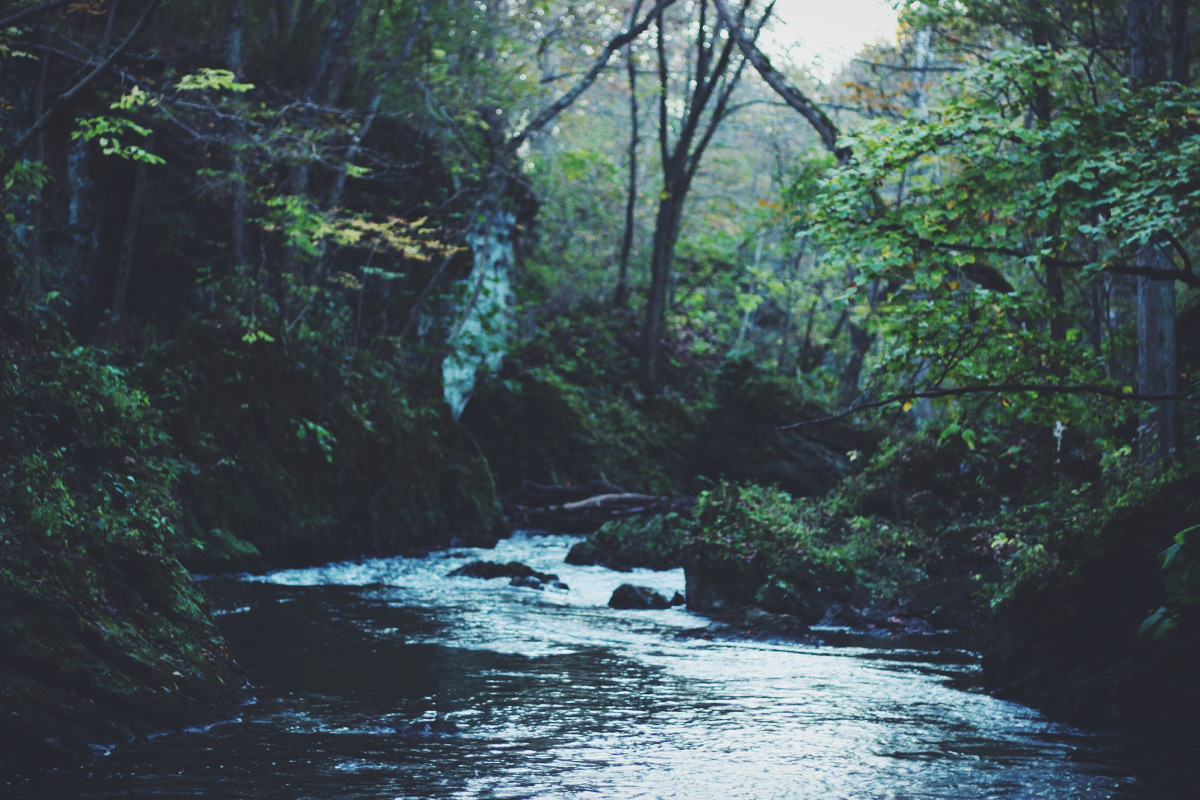
\includegraphics[width=\linewidth]{stream}
%%\caption{Legend (350 words max). Example legend text.}
%\label{fig:stream}
%\end{figure}

%\begin{table}[ht]
%\centering
%\begin{tabular}{|l|l|l|}
%\hline
%Condition & n & p \\
%\hline
%A & 5 & 0.1 \\
%\hline
%B & 10 & 0.01 \\
%\hline
%\end{tabular}
%\caption{\label{tab:example}Legend (350 words max). Example legend text.}
%\end{table}

%Figures and tables can be referenced in LaTeX using the ref command, e.g. Figure \ref{fig:stream} and Table \ref{tab:example}.

\end{document}
